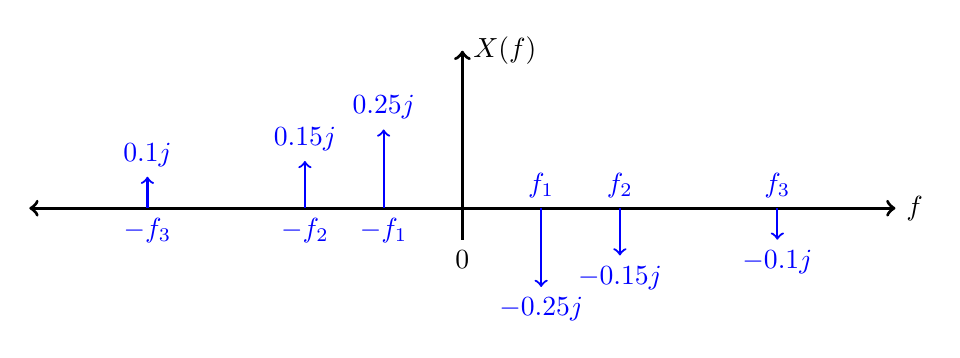
\begin{tikzpicture}[thick, y=4cm]
\draw[<->, very thick] (-5.5, 0) -- (5.5, 0) node[right]{$f$};
\draw[->, very thick] (0,-0.1) node[below]{$0$} -- (0, 0.5) node[right]{$X(f)$};

\foreach \f\x\l in {
    -4/0.1/$-f_3$,
    -2/0.15/$-f_2$,
    -1/0.25/$-f_1$,
    4/-0.1/$f_3$,
    2/-0.15/$f_2$,
    1/-0.25/$f_1$
} {
    \pgfmathparse{\x<0}
    \ifnum \pgfmathresult=1
        \draw[blue, ->] (\f,0) node[above]{\l} -- ++(0,\x) node[below]{$\x j$};
    \else
        \draw[blue, ->] (\f,0) node[below]{\l} -- ++(0,\x) node[above]{$\x j$};
    \fi
}

\end{tikzpicture}